\section{Experimental Evaluation}
\label{sec:eval}
We evaluated whether the runtime routed a request to the configured simulator setpoint, blocked inadmissible values, and made the resulting process measurements available to the caller. The endpoint probes exercise node mappings and their guards. The scripted runs use the agent-tool interface to alternate acquisition and recipe trials. Separate fixtures test approval and production-mode checks, and three language-model episodes show what the agent path completed.

The integrated runs used already-running services. Benchmark mode bypassed step, interval, and hold-window checks for agent and manual writes. We exercised those checks separately in production mode. All equipment responses reported here came from simulators or mock drivers.

\subsection{Configured Mapping and Integration Checks}
\label{sec:eval-mapping}
Two integrated executions at seed~42 each passed 77 assertions across 17 phases without an agent harness. A separate cast-film preset check on the same runtime configured five endpoint types and rejected all nine negative probes.

The retained November 6 matrix used the administrative node-write interface at 55 endpoints in four simulated scenes. It covered Modbus over Transmission Control Protocol (TCP), Modbus remote terminal unit (RTU), OPC UA, MQTT, and Hypertext Transfer Protocol (HTTP). Per endpoint, the runner submitted three interior values and the upper configured recipe-window bound, then tested values outside the recipe window and the hard engineering range. The common $-50$ candidate fell inside the biaxial dew-point range and was filtered before submission. The runner counted acceptance when the service returned HTTP~200 without an explicit unsuccessful outcome. On readable nodes, it issued a separate read after each admissible request and compared the simulator value with the request using the configured tolerance.

Table~\ref{tab:scene-probe-results} reports 220 accepted requests, 219 hard-range rejections, and 110 recipe-window rejections. Each of the 54 readable endpoints returned four distinct values in request order, for 216 matching readbacks. For example, the injection holding pressure read back 65~bar over OPC UA, the wastewater blower 35~Hz and the annealing zone~2 setpoint 725~$^\circ$C over Modbus TCP, and the biaxial drying setpoint 160~$^\circ$C over OPC UA. The corresponding injection probe at 102.8~bar was within the hard range and failed the recipe-window check. The one configured HTTP endpoint accepted all four corona-power requests, including 4.3~kW, and offered no actuator readback. Probe values and guards used the same scene configuration.

\begin{table*}[!t]
\centering
\caption{Outcomes of the retained scene--protocol probes. Denominators give the number of submitted probes or available follow-up reads in each class.}
\label{tab:scene-probe-results}
\footnotesize
\setlength{\tabcolsep}{3pt}
\begin{tabularx}{\textwidth}{@{}>{\raggedright\arraybackslash}p{1.55cm}r X r r r r@{}}
\toprule
Scene & Endpoints & Protocols represented & Accepted & Hard-range rejects & Recipe-window rejects & Matching reads \\
\midrule
Injection & 11 & TCP 5, RTU 2, OPC UA 3, MQTT 1 & 44/44 & 44/44 & 22/22 & 44/44 \\
Wastewater & 7 & TCP 1, RTU 3, OPC UA 2, MQTT 1 & 28/28 & 28/28 & 14/14 & 28/28 \\
Annealing & 7 & TCP 3, RTU 2, OPC UA 1, MQTT 1 & 28/28 & 28/28 & 14/14 & 28/28 \\
Biaxial line & 30 & TCP 20, RTU 1, OPC UA 8, HTTP 1 & 120/120 & 119/119 & 60/60 & 116/116 \\
\bottomrule
\end{tabularx}
\end{table*}

\subsection{Exploratory Fixed-Horizon Simulator Contrast}
\label{sec:eval-optimization}
We compared a deterministic setpoint policy with no-write in injection molding, wastewater treatment, and annealing. The script read the scene's configured DAQ variables, selected a candidate using scene-specific rules, and sent one recipe parameter per \texttt{recipe\_trial} call. The lines used automatic approval policy, with the applicable recipe checks and limits in force. The script logged trial requests and available recipe-run identifiers, allowed the process to settle, and used subsequent measurements to decide the next step.

The target bands were $32.5\pm0.35$~g for part mass, $3.4\pm0.6$~mg/L for dissolved oxygen, and $95\pm6$~HV for Vickers hardness. Runs used a nominal horizon of 180~s for injection and 240~s for the other scenes, with nominal 1-s sampling. Each arm had a separate reset and had to start within the prescribed process-value window. Arm order was randomized within each scene--seed block. We computed integrated absolute error (IAE) by trapezoidal integration of the absolute deviation from the target between the first and last retained samples. Internal gaps of up to 5~s were linearly interpolated. Longer gaps invalidated the pair.

Nine of the 11 blocks in the later post-pilot batch met the reset, start, and sampling criteria. Wastewater seed~45 and annealing seed~46 were excluded because their no-write traces had gaps of 9 and 6~s, respectively. The scripted policy had lower IAE in all nine valid pairs (Table~\ref{tab:selected-iae}). Each scripted run recorded a sample in its target band, and all nine no-write runs stayed outside their bands. Restricting each pair to its common observed time interval preserved the direction of all nine contrasts.

\begin{table}[!t]
\centering
\caption{Selected fixed-horizon simulator contrasts. Positive $\Delta$IAE means lower retained-window accumulated absolute error under the scripted policy.}
\label{tab:selected-iae}
\footnotesize
\setlength{\tabcolsep}{3pt}
\begin{tabular}{@{}lcc@{}}
\toprule
Scene (unit of $\Delta$IAE) & Valid & Median (range) \\
\midrule
Injection (g\,s) & 3/3 & 165.165 (162.535--195.169) \\
Wastewater ((mg/L)\,s) & 3/4 & 615.605 (611.670--630.980) \\
Annealing (HV\,s) & 3/4 & 8000.450 (7930.200--8084.150) \\
\bottomrule
\end{tabular}
\end{table}

The mission records show how the script used the route in each scene. At injection seed~44, it requested 58.31~bar from 45~bar and then 10.67~s from 6~s of holding time. The final post-settling mean was 32.163~g. At wastewater seed~43 the blower request went from 26 to 30.02~Hz, followed by further blower and dosing trials, and final dissolved oxygen was 3.620~mg/L. At annealing seed~43 the first zone~3 request went from 730 to 850~$^\circ$C. The script then adjusted zone~2 and line speed and recorded a final hardness of 98.92~HV. These sequences pair the script's recorded requests with its subsequent measurements. The archive lacks an aligned per-request driver journal for these runs.

Fig.~\ref{fig:optimization-trajectory}(a) shows that injection samples entered the target band within 15~s in all three scripted runs. Fig.~\ref{fig:optimization-trajectory}(b) lists their recorded starting and requested setpoints, including a second pressure request after the hold-time request for seed~46. Panels~(c)--(e) show the IAE for all nine valid pairs. An earlier valid injection seed-44 pair had an IAE difference of 193.320~g\,s, compared with 165.165~g\,s in the later repeat. The archive does not identify a pre-specified rule for choosing between batches. Supplementary File~S7 describes the exclusions and retained records.

\begin{figure*}[!t]
\centering
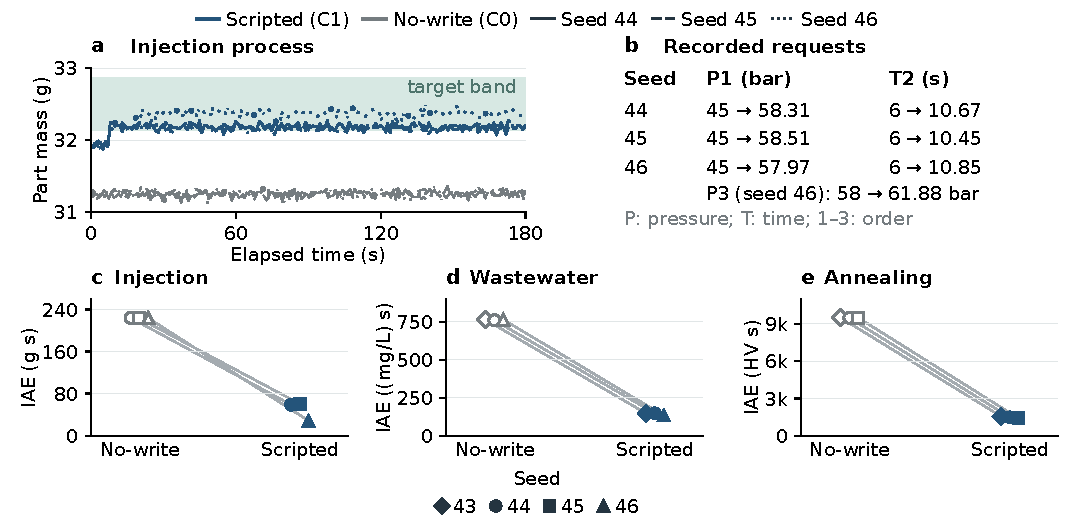
\includegraphics[width=\textwidth]{resources/fig5.pdf}
\caption{Scripted policy (C1) and no-write (C0) in the reported simulator batch. (a) Injection part-mass samples with the 32.15--32.85~g band shaded. Gaps over 1.5~s appear as breaks, and dots mark isolated samples. (b) Starting and requested setpoints from the script log. P and T denote hold pressure and hold time, and subscripts give request order. (c)--(e) Retained-window IAE for the nine valid pairs on scene-specific scales. Each line connects one seed pair. Small horizontal offsets separate overlapping markers.}
\label{fig:optimization-trajectory}
\end{figure*}

\subsection{Write-Guard and Route Behavior}
\label{sec:eval-ablation}
We tested the process-window check with a mock driver in one simulated scene. Four configurations combined enabled or disabled process-window and readback checks while retaining the hard range. Each configuration used three repetitions of four hard-range violations, two window violations, three legal values, and three boundary values. The violation values varied by configuration. Timed writes were counted separately.

Every configuration rejected all 12 hard-range violations and accepted all nine legal values. Enabling the window check rejected all six window violations per configuration. Disabling it let all six pass. Each configuration met all nine of its boundary expectations (Fig.~\ref{fig:guard-approval-results}(a)). This fixture measured service responses without injecting a readback mismatch.

A separate readback-fault probe returned 251 for a command of 230 with a tolerance of 0.7. The service returned HTTP~200 with an unsuccessful outcome graded \texttt{unverified}. A separate read of the simulator returned 251 as well. The baseline and recovery calls both returned \texttt{readback-verified}. In production mode, single tests of the interval, step, hard range, recipe window, and hold window all rejected the inadmissible request and the legal baseline passed. Authorization checks blocked unbound and cross-node requests and accepted the bound write.

The approval fixture submitted four \texttt{optimization\_explore} requests for injection barrel zone~1 temperature. A scripted approval permitted the setpoint to change from 202 to 204.8~$^\circ$C. A decline left it at 216~$^\circ$C. With approval disabled, the two requests changed 202 to 204.8~$^\circ$C and 216 to 218.8~$^\circ$C (Fig.~\ref{fig:guard-approval-results}(b)). The recorded pairing labels did not align with the starting temperatures, so we report the calls individually.

\begin{figure*}[!t]
\centering
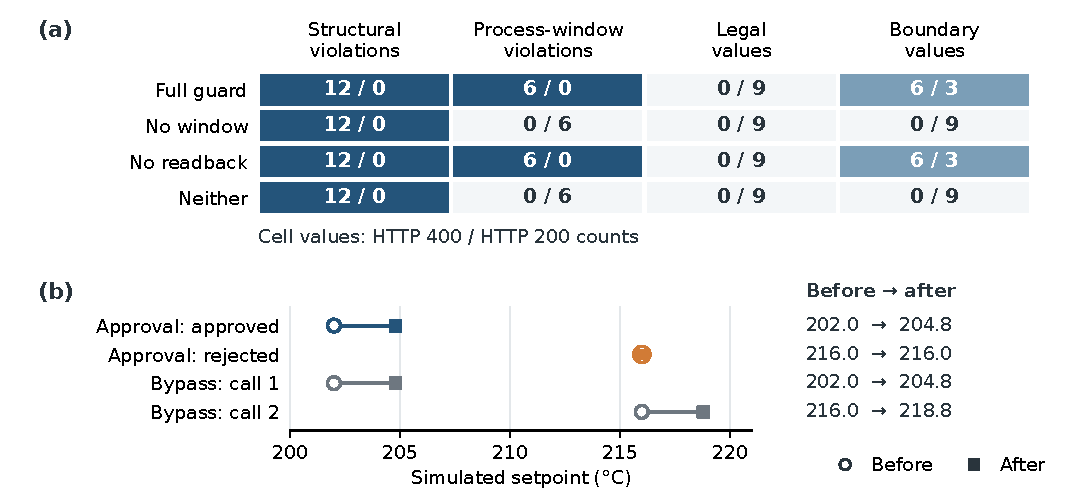
\includegraphics[width=\textwidth]{resources/fig6.pdf}
\caption{Guard and approval results. (a) HTTP~400/200 response counts for four guard configurations and four request classes. Shading gives the rejection proportion. Boundary expectations follow each configuration. (b) Simulated barrel-temperature setpoints before (circles) and after (squares) four separate requests. A scripted proxy supplied approval decisions where required.}
\label{fig:guard-approval-results}
\end{figure*}

\subsection{Injection-Twin Demonstration}
\label{sec:eval-twin-pilot}
An acceptance script submitted a three-step holding-pressure plan to an injection simulator. The execution service refused the pending plan until a scripted approval released it. After the three planned steps completed, a separate governed command changed holding pressure from 60 to 63.7~bar and the readback matched at 63.7~bar. After a 60-s wait, the last three 15-s DAQ buckets averaged 32.224~g, within the twin's 32.00--32.30~g band. Supplementary File~S7 records the baseline discrepancy and missing raw series for this single demonstration.

\subsection{LLM-Driven Simulator Episodes}
\label{sec:eval-agent}
Three injection episodes used the \texttt{deepseek-flash} model endpoint. Each worker trace contains a two-parameter recipe trial with automated approval and a response reporting both settings as verified. Separate episode-end platform snapshots show the same pressure and time values: 53~bar and 8~s, 54.8~bar and 8.2~s, and 56.6~bar and 8.4~s. The server-side driver journal and served model snapshot identifier were unavailable. All three tasks were canceled below the 32.15--32.85~g target band, at 31.70, 31.87, and 31.99~g, respectively. One episode recorded a process-quality guard flag.

